\chapter{Diseño}
\label{cap:capitulo4}

\begin{flushright}
\begin{minipage}[]{9cm}
\emph{El diseño no es solo lo que se ve y lo que se siente. El diseño es cómo funciona}\\
\end{minipage}\\

Steve Jobs, \textit{conferencia de lanzamiento del Apple iPod, 2001}\\
\end{flushright}

\vspace{1cm}

Después de definir la plataforma de desarrollo, se procede a explicar el diseño de la aplicación.

El proyecto se divide en cuatro scripts, el primero se utiliza para crear o registrar un paciente, el segundo lanza la GUI y controla los parámetros del juego, el tercero permite visualizar el comportamiento del paciente durante la terapia, y el cuarto es el propio juego.

\section{Interfaz de registro de un paciente}
\label{section:registro}

Este script permite gestionar un conjunto de datos, que identifican a un paciente, mediante una GUI.

En primer lugar, se importan las bibliotecas estádar, mencionadas en el capítulo anterior, como \verb|tkinter|, que se utiliza para crear la interfaz gráfica, \verb|csv| para guardar los datos en un archivo CSV para su posterior uso, y \verb|os| para interactuar con el sistema de archivos.

Se obtiene el directorio de inicio del usuario y se crea un directorio dentro de este, si no existe, bajo el nombre \textit{database}, donde se almacenan los ficheros con los datos de registro y análisis terapéuticos de cada paciente.

Se definen tres funciones principales que gestionan las operaciones de la GUI.
La función \verb|exit()| cierra la ventana pincipal de Tkinter, \verb|clear()| limpia los campos de entrada y texto, y \verb|savedata()| guarda los valores de los campos, valida que el ID sea un número y crea un subdirectorio bajo el nombre del ID, si no existe, donde guarda los datos en un archivo CSV llamado \verb|ID.csv|.
Si el archivo no existe, se escribe el encabezado utilizando \verb|writer.writeheader()|.
Los datos se escriben con \verb|csv.DictWriter| y son guardados como \verb|strings|.
Cada campo es un \verb|Entry| enlazado a una variable de tipo \verb|StringVar| y hacen referencia al nombre, apellido e ID del paciente, frecuencia, amplitud y perturbación de la señal que generará el brazo robótico al inicio de la terapia, nivel y progreso del juego y un espacio para que el doctor incluya observaciones.

Se crea una ventana principal con un título y tamaño fijo de 600x500 píxeles.

Los estilos visuales se configuran con \verb|ttk.Style| y se definen dos frames distintas, \verb|main_frame| se utiliza como contenedor de los campos de entrada y texto y \verb|button_frame| para agrupar la lógica de los botones.

Se crean dos botones, \textit{Save} llama a \verb|savedata()| para guardar los datos, que a su vez llama a \verb|clear()| para limpiar los campos una vez que estos se han almacenado, y el botón \textit{Exit} llama a \verb|exit()| que cierra la aplicación.

\verb|root.mainloop()| inicia el bucle de eventos de Tkinter y la interfaz está activa hasta que se cierra la ventana.

En el Código \ref{cod:codejemplo}, escrito en \texttt{Python}, se muestra cómo se gestionan los directorios y la escritura del archivo CSV.

\begin{code}[h]
\begin{lstlisting}[language=Python]
def savedata():
    ID_DIR = os.path.join(DATABASE_DIR, id)
    os.makedirs(ID_DIR, exist_ok=True)
    file_name = f"{id}{ext}"
    file_path = os.path.join(ID_DIR, file_name)

    # [...]

    file_exists = os.path.isfile(file_path)
    with open(file_path, mode="a", newline="") as file:
        writer = csv.DictWriter(file, fieldnames=patient_data.keys())
        if not file_exists:
            writer.writeheader()
        writer.writerow(patient_data)
\end{lstlisting}
\caption[Función para guardar los datos de un paciente]{Función para guardar los datos de un paciente}
\label{cod:codejemplo}
\end{code}

En la Imagen \ref{fig:database} puede observarse el estilo de la interfaz.

\begin{figure}[ht!]
	\centering
	\begin{minipage}{0.75\linewidth}
		\centering
		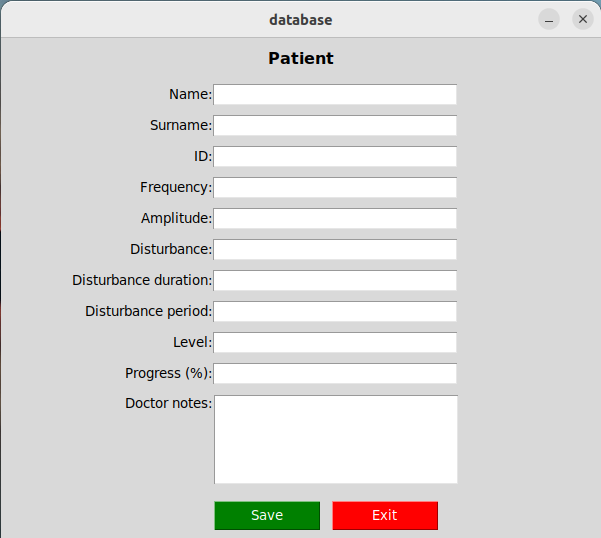
\includegraphics[width=\linewidth]{figs/registro.png}
	\end{minipage}
	\caption[Interfaz de registro de un paciente]{Interfaz de registro de un paciente}
	\label{fig:database}
\end{figure}

\section{Interfaz de control}
\label{section:controller}

Este script combina ROS 2 y Tkinter para crear una GUI que gestiona límites físicos (mínimo, máximo y offset) del robot, configura y publica parámetros para crear una señal de control y perturbación para un sistema robótico, parámetros de asistencia y nivel de dificultad para un videojuego terapéutico y almacena dichas configuraciones por paciente.

Al inicio del script se importan las librerías \verb|rclpy|, que es la API cliente de Python para ROS 2, \verb|tkinter| para crear la interfaz gráfica, \verb|std_msgs.msg| para gestionar los mensajes estándar de ROS 2, \verb|csv| para el manejo de archivos CSV, \verb|os| para interactuar con el sistema y \verb|datetime| para gestionar la fecha de creación de los archivos.

Se crea un directorio en el directorio de inicio del usuario, si no existe, bajo el nombre \textit{database}, donde se almacenan los ficheros con los datos de configuración de cada paciente.

Se definen dos clases, \verb|ScrollPublisherNode| es una clase de ROS 2 que publica los parámetros de una señal (frecuencia, amplitud, offset y tipo) y de una perturbación (amplitud, duración, periodo y tipo).
Los datos se publican cada 0.1 segundos y son de tipo \verb|float|.
El tipo de señal y perturbación se codifica como 1.0 (sinusoidal) y 2.0 (escalón).
\verb|ScrollGUI| es la clase que crea la interfaz gráfica y permite ajustar los parámetros del juego en tiempo real y publicarlos a través de un nodo de ROS.
Los datos se guardan en un archivo CSV bajo el nombre \verb|ID-year-month-day-config_<index>.csv| en un subdirectorio llamado \textit{config} dentro del directorio \textit{home/user/database/ID/}.
\verb|index| hace referencia al número de archivo de la sesión diaria.
Si el archivo no existe, se escribe el encabezado.

Se crean deslizadores, utilizando \verb|ttk.Scale|, para ajustar la frecuencia, amplitud, offset, duración, periodo y asistencia del robot.
Se utiliza \verb|Combox| para permitir la selección entre los distintos tipos de señal y perturbación (sinusoidal o escalón) y niveles del juego (del 1 al 10).
Los botones \textit{Update Signal} y \textit{Update levels} se utilizan para publicar datos en los topics \verb|/SliderParameters| y \verb|/GameParameters|, respectivamente, y el botón \textit{Exit} para salir.

La función \verb|saveconfig()| guarda la configuración actual de la GUI en el archivo CSV.
Todas las funciones \verb|update*()| convierten el valor del deslizador de \verb|str| a \verb|float|.
Entre ellas se destacan \verb|updatesignal()|, que actualiza los atributos del nodo y llama a \verb|saveconfig()|, que añade al final del archivo la nueva configuración, y \verb|updatelevel()|, que publica un mensaje \verb|Int32MultiArray| con los datos de asistencia y nivel de dificultad del juego.
La función \verb|close()| finaliza el nodo y cirra la GUI y el método \verb|run()| inicia el bucle de eventos de Tkinter juto con el \verb|spin_once()| de ROS 2.
\verb|loadcsv()| lee el último registro del archivo del paciente que se pasa como parámetro y devuelve los valores de frecuencia, amplitud, perturbación, dureción, periodo y nivel del juego.
Todos son \verb|float| excepto el último que es un \verb|int|.

\verb|main()| es la función principal y se encarga de extraer el ID del paciente desde la ruta al archivo de registro, cargar los datos de las señales y el juego desde el CSV, crear el nodo \verb|ScrollPublisherNode| con dichos parámetros e iniciar la GUI.
\verb|startgui()| es la primera interfaz que se lanza y gestiona la configuración de los límites físicos del robot a través de la publicación de un \verb|Int32MultiArray| que actúa como un booleano indicando el botón que se ha pulsado (resetear, mínimo, máximo, offset o continuar).
Además, comprueba que los límites mínimo y máximon se han definido correctamente antes de permitir establecer el offset o continuar a la siguiente ventana.

En la Imagen \ref{fig:config} se muestra la ventana de inicio y en la Imagen \ref{fig:control} la ventana principal.

\begin{figure}[ht!]
	\centering
	\begin{minipage}{0.85\linewidth}
		\centering
		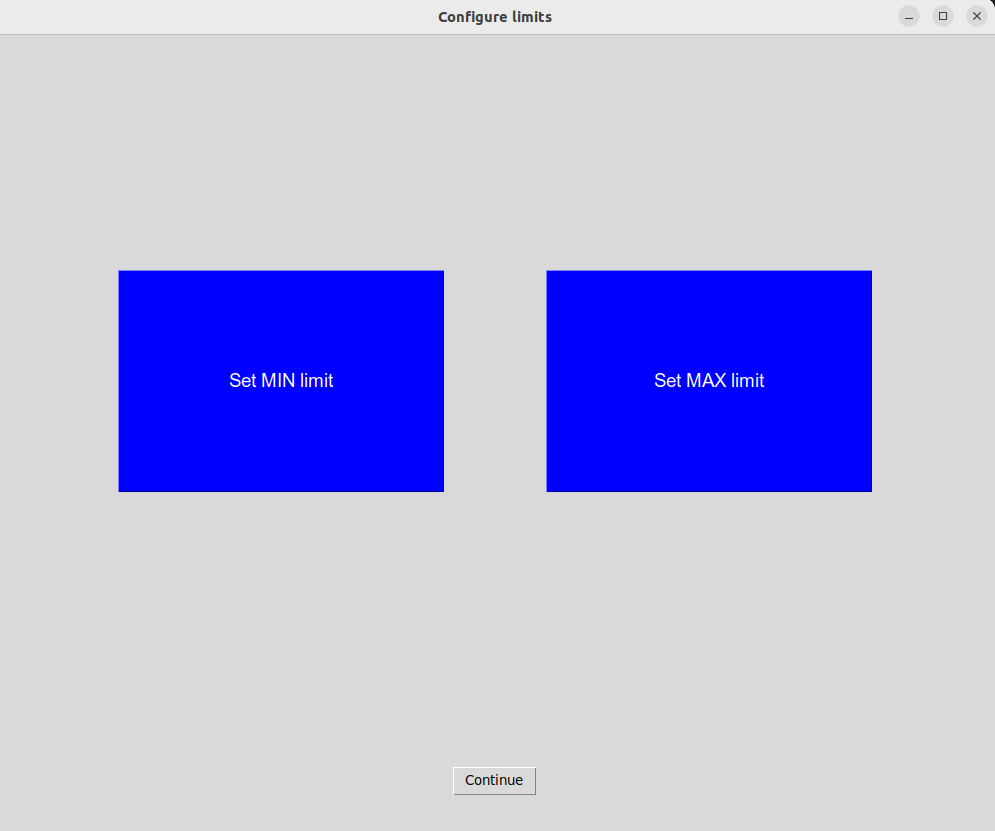
\includegraphics[width=\linewidth]{figs/config_limits.png}
	\end{minipage}
	\caption[Interfaz de configuración de los límites del brazo robótico]{Interfaz de configuración de los límites del brazo robótico}
	\label{fig:config}
\end{figure}

\begin{figure}[ht!]
	\centering
	\begin{minipage}{0.85\linewidth}
		\centering
		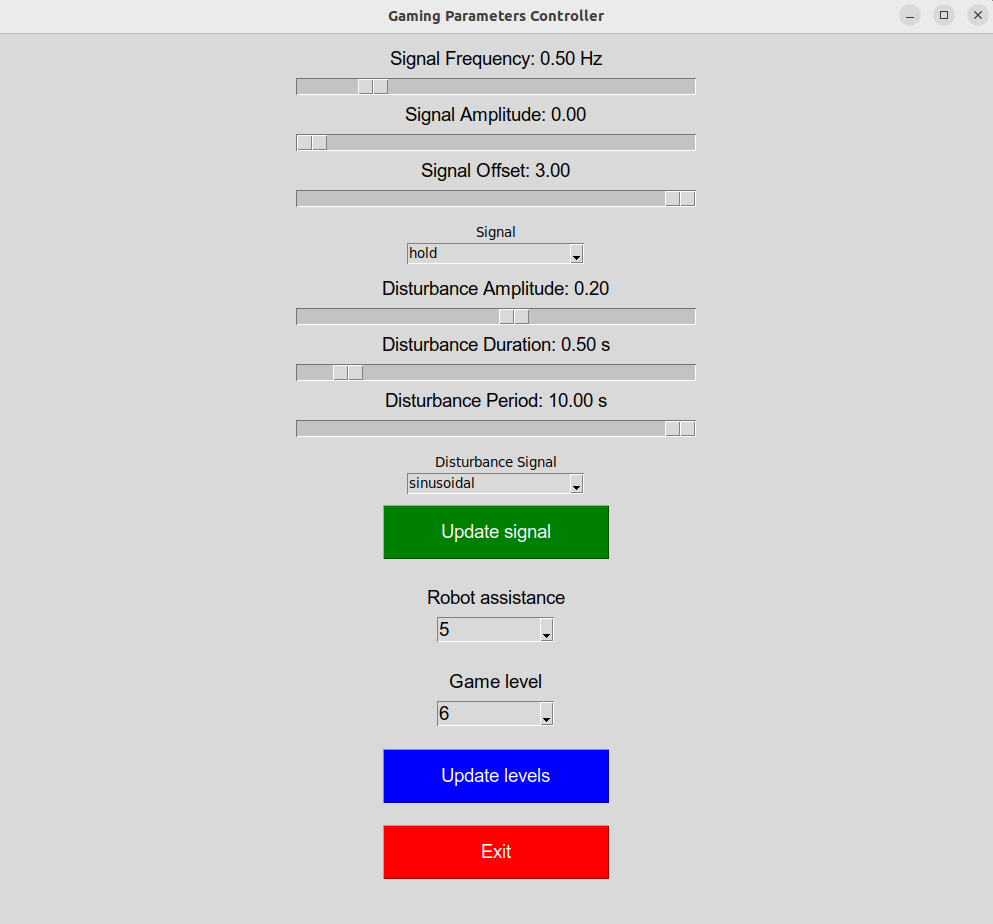
\includegraphics[width=\linewidth]{figs/control_pannel.png}
	\end{minipage}
	\caption[Interfaz de control]{Interfaz de control}
	\label{fig:control}
\end{figure}

\section{Interfaz de visualización}

Este script permite observar y registrar la ejecución de un paciente en una tarea de seguimiento de trayectoria como parte de una sesión de rehabilitación motora.

A parte de utilizar las bibliotecas mencionadas en la Sección \ref{section:controller}, se utilizan \verb|matplotlib| para visualizar los datos del rendimiento del jugador en tiempo real, \verb|numpy| para manejar los datos de las señales que cambian con el tiempo y \verb|sys| para gestionar la ruta al archivo CSV con los datos de registro del paciente.

Se utiliza el modo interactivo de \verb|matplotlib|, \verb|plt.ion()|, que permite actualizar dinámicamente los gráficos sin bloquear el hilo principal.
Las ventanas son deslizantes, no obstante debemos mantener un tamaño fijo para que la señal no se desplace hacia la izquierda, por ello se implementa \verb|np.roll()|.

Se define la clase \verb|FlappyBirdViewerNode| que actúa como nodo de ROS 2 y se suscribe a los topics \verb|/ClanSignal|, donde se publica la señal de referencia que se toma como trayectoria deseada que el jugador debe seguir, \verb|/Disturbance|, que contiene la señal de perturbación y \verb|/PlayerPosition|, que tiene información de la posición del jugador y del desplazamiento vertical de la señal.
\verb|signalcallback()| se activa cada vez que se recibe un valor de la señal, si el jugador está activo se actualizan los datos (tiempo, límites, posición, error de trayectoria y detección de colisiones) y se grafican.
Para la detección de colisiones se implementa una lógica simple basada en la comparación de la posición del jugador con los límites de la señal.
\verb|playercallback()| actualiza la posición del jugador, el offset que separa la señal de los límites y el tiempo total y marca que el jugador está activo.

Se muestran dos gráficos, el que está en la parte superior permite visualizar la señal principal, la perturbación, los límites superior e inferior y la posición actual del jugador.
Y, la parte inferior grafica el error de posición con respecto a la trayectoria deseada en función del tiempo, lo que permite detectar fallos de control, fatiga o pérdida de atención.

Para ello se utiliza la Ecuación \ref{ec:ec1}.

\begin{myequation}[h]
\begin{equation}
error(t) = | y_{player}(y) - y_{reference}(t) |
\nonumber
\label{ec:ec1}
\end{equation}
\caption[Cálculo del error de trayectoria]{Cálculo del error de trayectoria}
\end{myequation}

Al finalizar la ejecución, los datos más relevantes como el tiempo, la señal, los límites mínimo y máximo, la posición del jugador, el offset, el error y las colisiones se almacenan en un archivo CSV bajo el nombre \verb|ID-year-month-day-metrics_<index>.csv| en un subdirectorio llamado \textit{metrics} dentro del directorio \textit{home/user/database/ID/}.
\verb|index| hace referencia al número de archivo de la sesión diaria.
Esto facilita un análisis posterior de la terapia.

La función principal \verb|main()| verifica que se ha pasado como único argumento un archivo CSV con los datos de registro del paciente, extrae el ID desde la ruta, crea el nodo \verb|FlappyBirdViewerNode| y escucha de los topics.

En la Imagen \ref{fig:visual} se puede visualizar la retroalimentación obtenida durante la terapia.

\begin{figure}[ht!]
	\centering
	\begin{minipage}{0.85\linewidth}
		\centering
		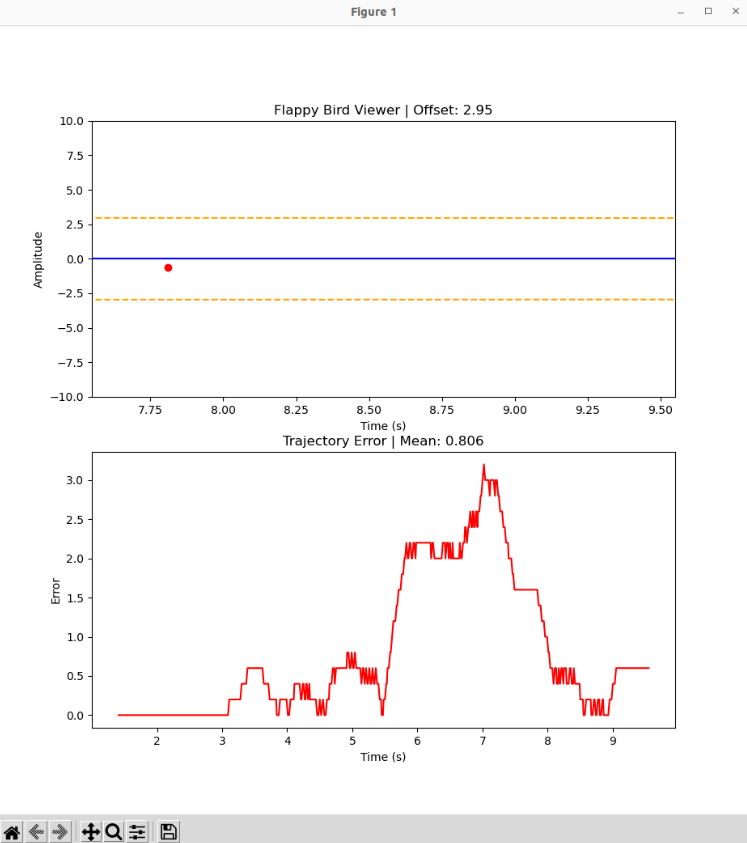
\includegraphics[width=\linewidth]{figs/visual.png}
	\end{minipage}
	\caption[Interfaz de visualización]{Interfaz de visualización}
	\label{fig:visual}
\end{figure}

\section{Juego flappy}
